\chapter[Analiza problemu]{Analiza problemu}

\label{analiza_problemu}

% W tym rozdziale trzeba bardziej szczegółowo opisać jak chce Pan
% zrealizować cele sformułowane w rozdziale 2.
% Jakie będą konsekwencje i ewentualne wyzwania techniczne
% związane z przyjętą strategią. Jaka ogólnie ma być komunikacja
% z komputerem, tzn. czy to ma być tryb pytanie-odpowiedź, czy ciągłe
% przesyłanie danych. Czy być może jakiś tryb mieszany.
% Jaką chce Pan przyjąć formę przetwarzania danych i dlaczego. itd. itd.


\section{Plan urządzenia}

Założenia konstrukcyjne to przede wszystkim prostota budowy, modularność i skrócenie czasu realizacji. 
Płytka deweloperska wysyła określoną przez użytkownika liczbę przebiegów sygnału PWM
\footnote[1]{Pulse Width Modulation ang. Modulacja Szerokości Impulsów}, następnie sygnał jest ten wzmacniany 
do poziomu aż 80 woltów by uzyskać maksymalną wydajność i trafia na przetwornik piezoelektryczny który generuje falę ultradźwiękową.
Fala ta po odbiciu się od obiektu w polu wykrywania sonaru trafia z powrotem do urządzenia a konkretniej do mikrofonów MEMS umieszczonych na czole obudowy.
Sygnał z mikrofonów jest filtrowany by przepuścić tylko porządane przez nas częstotliwości bliskie czestotliwości nadajnika, 
oraz wzmacniany w celu lepszej interpretacji przez dalsze układy.
Po przefiltrowaniu, sygnał jest progowany. Mikrokontroler za pomocą przetwornika DAC ustala poziom napięcia, 
który wyznaczy granicę pomiędzy wysokim a niskim stanem logicznym. To rozróznienie jest nam potrzebne do pobudzenia cyfrowego wejścia licznika, 
zmienność tej wartości pozwala nam również na reagowanie tylko na sygnał o odpowiedniej amplitudzie by móc z powrotem obniżyć próg 
do miejsca przecięcia się sinusoidy z napięciem odniesienia, gdzie dokładność pomiaru jest największa.
Mikroprocesor dzięki wspomnianym wcześniej licznikom odmierza czas między zboczami rosnącymi zprogowanego już sygnału.
Wszystkie pomiary czasów przecieć z trzech odbiorników są wysyłane we wspólnej ramce danych do komputera gdzie za pomocą 
różnic w tych czasach wyznaczony zostanie dystans obiektu oraz jego odchylenie względem sonaru.
\begin{figure}[ht!]
    \centering
    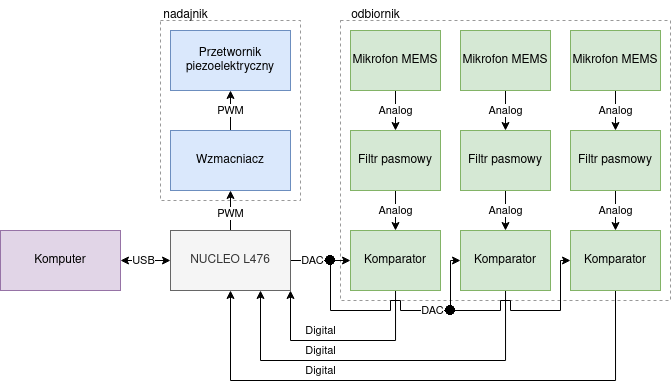
\includegraphics[width = 0.8\textwidth]{sonar_uml.png}
    \caption{Schemat blokowy urządzenia}
    \label{fig:uml}
\end{figure}



\section{Rozmieszczenie elementów nadawczych i odbiorczych}
Rozmieszczenie odbiorników jest kluczowym elementem pomiaru, to dzięki znajomości odległości mikrofonów i różnic w czasach 
dotarcia sygnału jesteśmy w stanie określić kąt pod którym fala dźwiękowa trafia do urządzenia. Do uzyskania pełnego zakresu 

\begin{figure}[ht!]
    \centering
    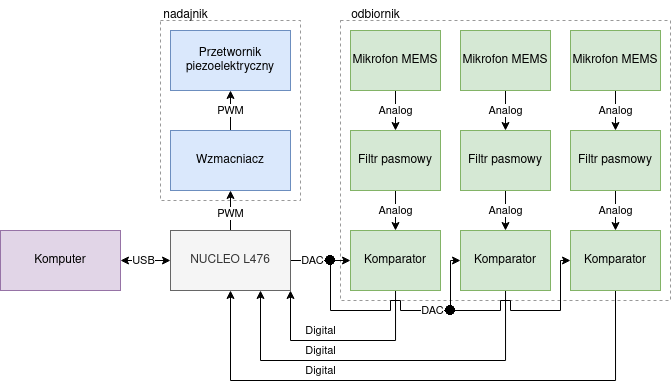
\includegraphics[width = 0.5\textwidth]{sonar_uml.png}
    \caption{Schemat blokowy urządzenia}
    \label{fig:uml}
\end{figure}



\section{Komunikacja}


\section{Przetwarzanie danych}